\section{Introduction}
\label{sec:introduction}

Human dexterity relies fundamentally on the seamless integration of high-frequency tactile mechanoreception, proprioceptive joint sensing, and anticipatory motor control. When a person carries a fragile glass vessel being filled with liquid while navigating over uneven terrain, optical and dermal mechanoreceptors detect infinitesimal shear strains and incipient slip tens of milliseconds before gross sliding occurs \cite{pandas2024incipient,shear2025grasp}. This biological pre-slip signal allows the central nervous system to modulate grip forces proactively, stabilizing dynamic payloads without exceeding the fracture threshold of the object.

In autonomous robotics, replicating this dexterous compliance has proven elusive. Modern robotic systems face a persistent trilemma during contact-rich physical interactions:
\begin{enumerate}
    \item \textbf{Generative Vision-Language-Action (VLA) Policies:} Recent foundation models, such as $\pi_0$ \cite{pi02024}, OpenVLA \cite{openvla2024}, and TacClaw-Infinity \cite{tacclaw2026infinity}, demonstrate broad semantic task generalization. However, they typically output actions via unconstrained flow matching or diffusion decoders at modest control frequencies ($5\text{--}10\text{ Hz}$). When unanticipated contact nonstationarities arise (e.g., condensation, fluid spills, or mass shifts), these generative policies cannot alter internal joint torques within the necessary sub-step timescale ($10\text{ ms}$), frequently breaching contact friction cones.
    \item \textbf{Reactive Grip Reflexes:} Classical industrial controllers implement local reflexive squeeze rules that monitor high-frequency tactile slips. However, because they trigger only \emph{after} macroscopic sliding has initiated, the accelerated payload often escapes the fingertip friction envelope before finger actuators can overcome mechanical inertia and build normal force.
    \item \textbf{Certainty-Equivalence Model Predictive Control (CE-MPC):} Optimization-based force controllers solve receding-horizon quadratic programs to track contact wrenches. However, they rely on deterministic friction coefficients. Under sudden environmental shifts, point estimators lag behind physical reality, allowing the commanded force vector to penetrate the true friction boundary.
\end{enumerate}

\begin{figure}[t]
    \centering
    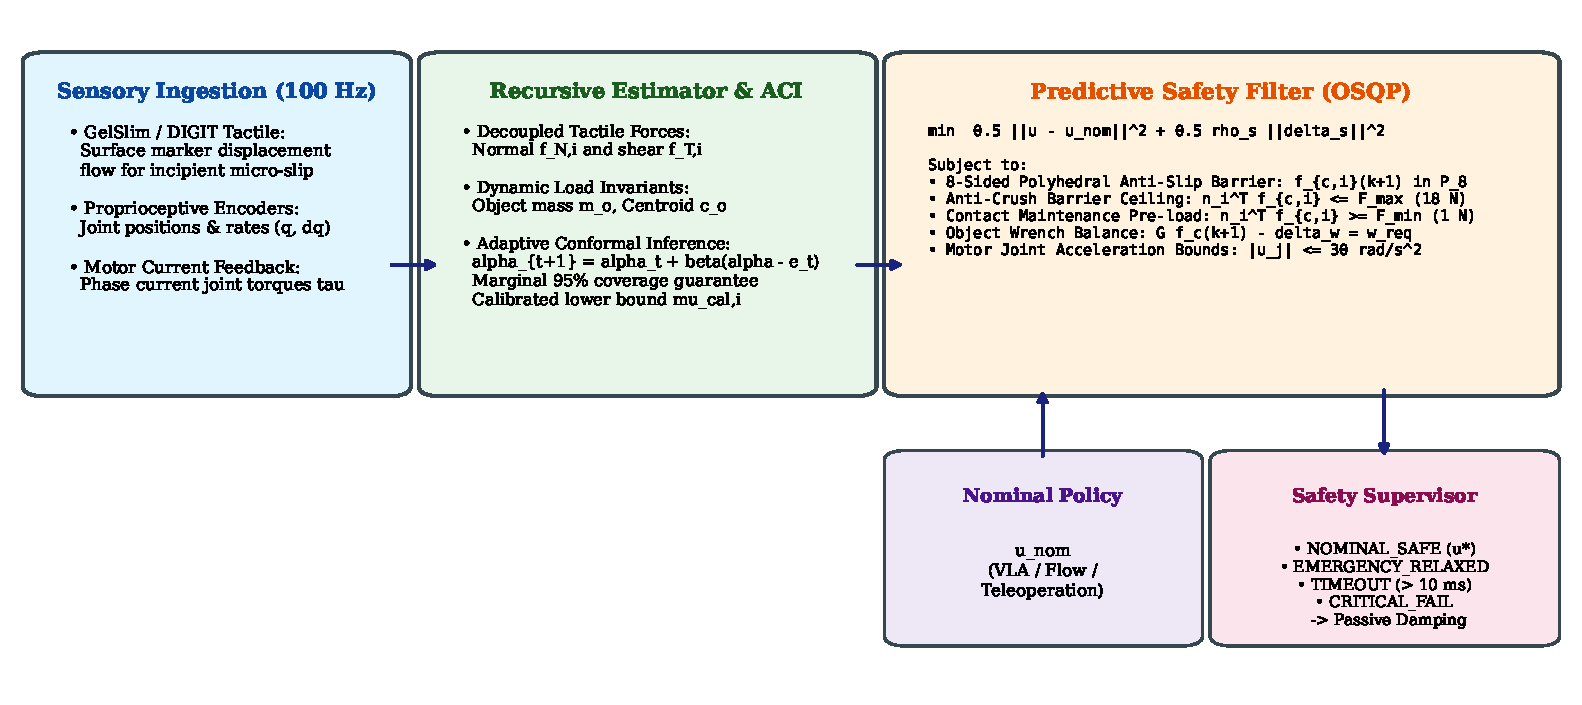
\includegraphics[width=\textwidth]{figures/architecture.pdf}
    \caption{\textbf{HOROS PROBE-1 System Architecture.} High-speed sensory modalities (100~Hz optical tactile flow, joint encoders, and motor effort) feed a recursive multi-contact estimator. Adaptive Conformal Inference (ACI) tracks non-exchangeable friction shifts to yield dynamically calibrated bounds $\mu_{\text{cal}}$. The predictive safety filter (OSQP) maps nominal policy actions $\mathbf{u}_{\text{nom}}$ to certified safe commands $\mathbf{u}^*$ via an 8-sided polyhedral inner approximation $\mathcal{P}_8$ and object wrench equilibrium, evaluated by a 4-state real-time decision gate.}
    \label{fig:architecture}
\end{figure}

To resolve this trilemma, this paper introduces \textbf{HOROS PROBE-1}, a predictive contact safety architecture designed for multi-fingered robotic hands operating under coupled nonstationary conditions. As illustrated in \Cref{fig:architecture}, our framework couples physics-grounded contact mechanics with non-exchangeable uncertainty calibration.

\subsection{Primary Contributions}
The core contributions of this work are summarized as follows:
\begin{enumerate}
    \item \textbf{Action-Dependent Contact Sensitivity Mapping:} We derive an analytical sensitivity tensor $\mathbf{\Lambda}_i(\mathbf{q}) \in \mathbb{R}^{3 \times n_q}$ mapping commanded joint accelerations $\mathbf{u}_k = \ddot{\mathbf{q}}_k$ directly to forward contact force evolutions $\mathbf{f}_{c, i}(k+1)$ based on linearized Hunt-Crossley elastomeric dynamics, ensuring direct control authority over the barrier constraints.
    \item \textbf{8-Sided Polyhedral Discrete-Time p-CBF:} We formulate an 8-sided polyhedral inner approximation $\mathcal{P}_8$ of the Lorentz friction cone that integrates seamlessly into a convex Quadratic Program (QP), with an analytical conservatism bound of $1 - \cos(\pi/8) \approx 7.61\%$.
    \item \textbf{Object-Level Spatial Wrench Equilibrium:} We project the multi-contact grasp matrix $\mathbf{G} \in \mathbb{R}^{6 \times 3M}$ directly into the equality constraint manifold, ensuring that internal grip force adjustments reside strictly within the grasp nullspace $\mathcal{N}(\mathbf{G})$, eliminating unwanted parasitic object accelerations.
    \item \textbf{Adaptive Conformal Friction Tracking:} We deploy Adaptive Conformal Inference (ACI) to maintain long-run average coverage ($1 - \alpha = 95.0\%$) over non-exchangeable, nonstationary friction shifts, providing calibrated uncertainty intervals $[\mu_{\text{cal}}, \mu_{\max}]$ directly to the barrier constraints.
    \item \textbf{Large-Scale Empirical Verification:} Across 3,400 independent simulation trials ($N = 100$ independent seeds per condition) in Isaac Lab with PhysX 5 continuous collision detection, HOROS maintains a \textbf{0.0\% drop rate and 0.0\% crush rate} under coupled nonstationarity, whereas all baselines suffer a \textbf{100.0\% drop rate} ($p < 10^{-20}$).
    \item \textbf{Separation of Slip and Structural Safety:} Systematic 7-component ablations demonstrate that joint proprioception and upper CBF bounds are strictly mandatory to prevent object destruction (100.0\% crush rate when ablated), proving that slip avoidance and fragile structural preservation are competing physical objectives.
\end{enumerate}
